\documentclass[tikz,border=5pt]{standalone}
\usepackage{tikz}
\usetikzlibrary{shapes,arrows,positioning,fit,backgrounds,calc}
\usepackage{amsmath}
\usepackage{amssymb}

\definecolor{semantic_low}{RGB}{200,230,200}  % light green
\definecolor{semantic_high}{RGB}{255,200,200} % light red
\definecolor{structural_low}{RGB}{200,220,255} % light blue
\definecolor{structural_high}{RGB}{255,230,180} % light orange
\definecolor{danger}{RGB}{220,50,50}
\definecolor{safe}{RGB}{50,150,50}
\definecolor{warning}{RGB}{220,150,50}

\begin{document}
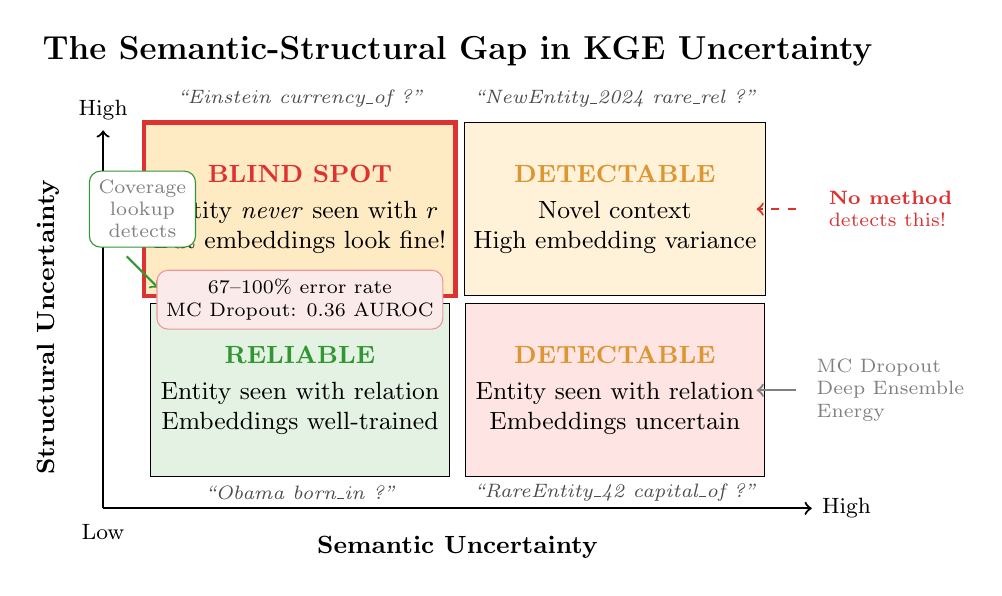
\begin{tikzpicture}[
    box/.style={rectangle, draw, minimum width=3.8cm, minimum height=2.2cm, align=center, font=\small},
    label/.style={font=\footnotesize\bfseries},
    method/.style={font=\scriptsize, text=gray},
    example/.style={font=\scriptsize\itshape, text=black!70},
]

% Title
\node[font=\large\bfseries] at (4, 5.5) {The Semantic-Structural Gap in KGE Uncertainty};

% Axis labels
\node[font=\small\bfseries, rotate=90] at (-1.2, 2) {Structural Uncertainty};
\node[font=\small\bfseries] at (4, -0.8) {Semantic Uncertainty};

% Axis arrows
\draw[->, thick] (-0.5, -0.3) -- (8.5, -0.3) node[right, font=\footnotesize] {High};
\draw[->, thick] (-0.5, -0.3) -- (-0.5, 4.5) node[above, font=\footnotesize] {High};
\node[font=\footnotesize] at (-0.5, -0.6) {Low};

% Quadrant 1: Low Semantic, Low Structural (SAFE)
\node[box, fill=semantic_low!50] (q1) at (2, 1.2) {
    \textcolor{safe}{\textbf{RELIABLE}}\\[2pt]
    Entity seen with relation\\
    Embeddings well-trained
};
\node[example] at (2, -0.1) {``Obama born\_in ?''};

% Quadrant 2: High Semantic, Low Structural (DETECTABLE)
\node[box, fill=semantic_high!50] (q2) at (6, 1.2) {
    \textcolor{warning}{\textbf{DETECTABLE}}\\[2pt]
    Entity seen with relation\\
    Embeddings uncertain
};
\node[example] at (6, -0.1) {``RareEntity\_42 capital\_of ?''};

% Quadrant 3: Low Semantic, High Structural (BLIND SPOT!)
\node[box, fill=structural_high!80, line width=1.5pt, draw=danger] (q3) at (2, 3.5) {
    \textcolor{danger}{\textbf{BLIND SPOT}}\\[2pt]
    Entity \emph{never} seen with $r$\\
    But embeddings look fine!
};
\node[example] at (2, 4.9) {``Einstein currency\_of ?''};

% Quadrant 4: High Semantic, High Structural (DETECTABLE)
\node[box, fill=structural_high!50] (q4) at (6, 3.5) {
    \textcolor{warning}{\textbf{DETECTABLE}}\\[2pt]
    Novel context\\
    High embedding variance
};
\node[example] at (6, 4.9) {``NewEntity\_2024 rare\_rel ?''};

% Method coverage annotations
\node[method, align=left] at (9.5, 1.2) {MC Dropout\\Deep Ensemble\\Energy};
\draw[->, gray, thick] (8.3, 1.2) -- (7.8, 1.2);

\node[method, align=left, text=danger] at (9.5, 3.5) {\textbf{No method}\\detects this!};
\draw[->, danger, thick, dashed] (8.3, 3.5) -- (7.8, 3.5);

% Coverage detection annotation
\node[method, align=center, fill=white, draw=safe, rounded corners] at (0, 3.5) {Coverage\\lookup\\detects};
\draw[->, safe, thick] (-0.2, 2.9) -- (0.2, 2.5);

% Stats annotation
\node[font=\scriptsize, align=center, fill=danger!10, rounded corners, draw=danger!50] at (2, 2.35) {
    67--100\% error rate\\
    MC Dropout: 0.36 AUROC
};

\end{tikzpicture}
\end{document}
